\section{Results}

The results section includes three topics: model validation and estimation, and estimation validation. In the model validation section we demonstrate that the neural mass model can mimic the dynamics observed in hippocampal seizure EEG. For the model estimation section we show that the unscented Kalman filter can be used to track changes in the synaptic gains and input mean of a neural mass model with EEG observations. In the estimation validation section, we then explore how descriptive the model estimates are of the recorded EEG. This is achieved by simulating data using the estimated synaptic gains and mean input firing rate. The simulated data is then compared to the recorded EEG to determine whether the estimates are capable of replicating the key characteristics observed.

\subsection{Model Selection}

The neural mass model of the hippocampus has been shown to be capable of replicating the frequency dynamics of hippocampal EEG~\citep{wendling2002epileptic}. In Figure~\ref{fig: EEG} two EEG traces are demonstrated, the first of recorded EEG from a rat that has had tetanus toxin injected into its hippocampus, and the second of simulated data using the Wendling model. The simulated data is generated by altering the synaptic gains and the input mean of the Wendling model. In both traces the red dashed lines indicate the beginning and end of a seizure. Their is a clear relationship between the amplitude of the simulated data and the recorded EEG. In particular, at seizure onset the amplitudes of the simulated and recorded data increase. Prior to seizure termination their is a marked decrease in amplitude in both the recorded and simulated data.
 
Even though their are clear similarities between the two traces, their are also clear differences. These differences are due to the input to the neural mass model, which is stochastic, and unknown for the recorded EEG. However, using this technique we can extract the underlying structural dynamics buried in the intracranial EEG. In this study, we evaluate the most likely set of physiological parameters that describe the transitions between seizure and non-seizure, and how they alter during seizure.

\begin{figure}[ht]
 	\centering
 		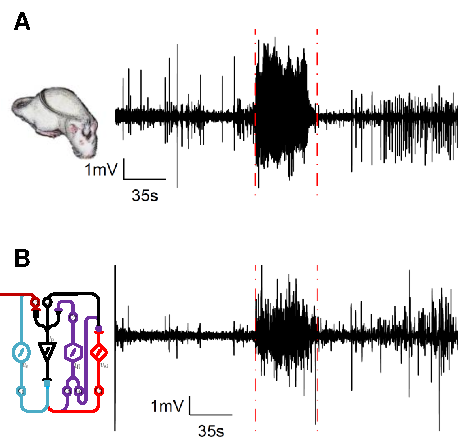
\includegraphics{fig/EEG.pdf}
 	\caption{Recorded and Simulated EEG. (\textbf{A}) Recorded intracranial EEG from the hippocampus of a rat that has had a tetanus toxin injection. (\textbf{B}) Simulated data generated from the neural mass model of the hippocampus. The red dotted lines indicate the start and end of a seizure in both traces.}
 	\label{fig: EEG}
 \end{figure}

\subsection{Estimation}

Hippocampal EEG can be mimicked by altering the synaptic gains of the neural mass model. As a further addition, we also consider the mean input firing rate to the modeled neural mass to be time varying. For this study, we have used recordings from four different control animals, and consider four seizures from each of them. All parameters are initialised identically and the same algorithm is used for all recordings. 
\begin{figure}[ht]
 	\centering
	 \vspace*{-4cm}
 		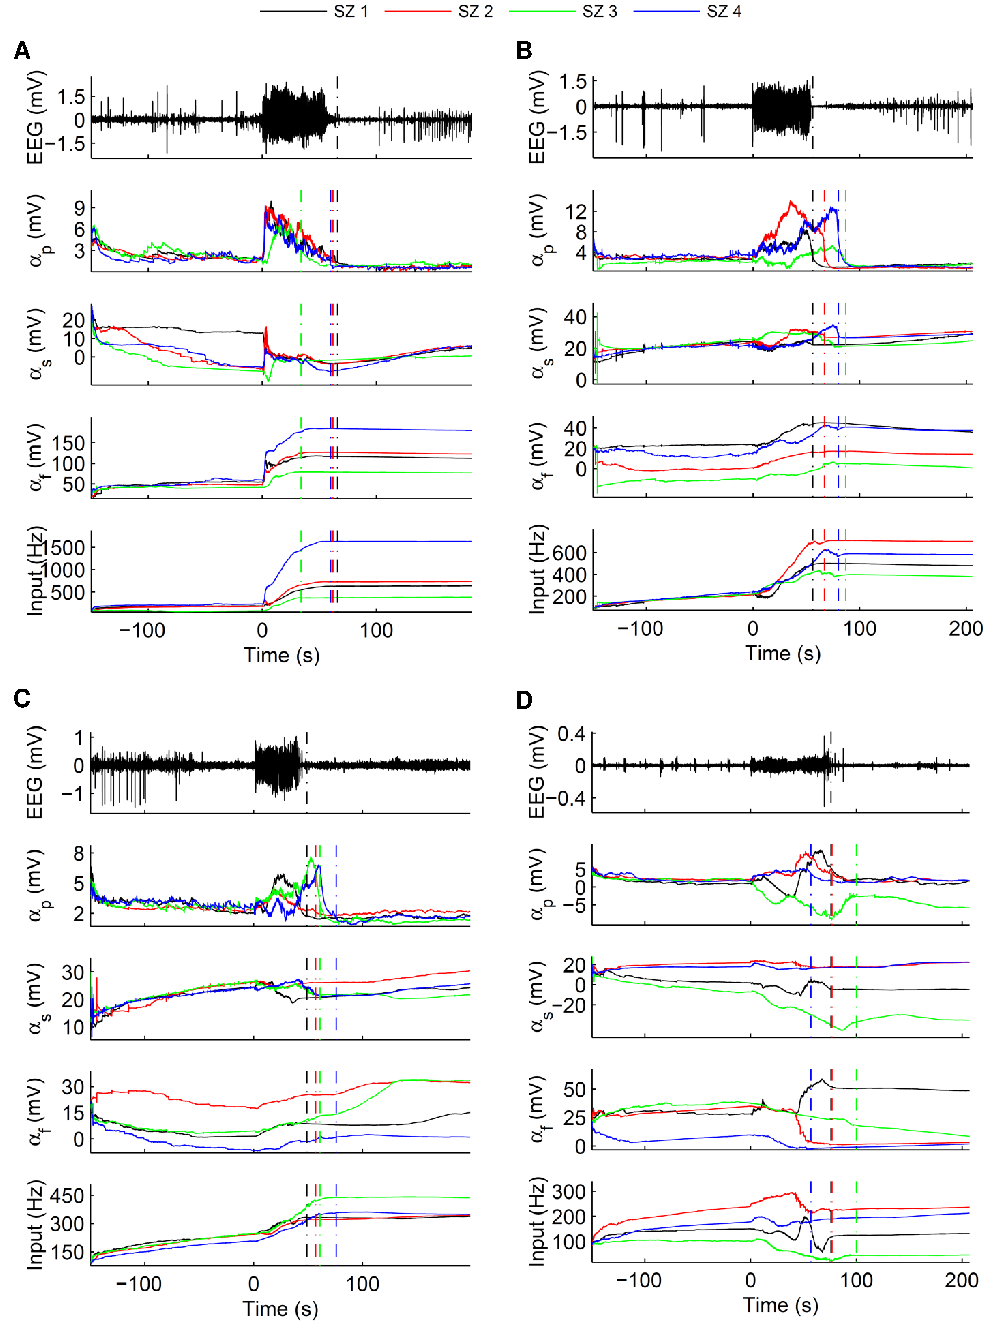
\includegraphics[max size={\textwidth}{\textheight}]{fig/EstimationFigures1.pdf}
 	\caption{Results from the estimation of four seizures from four different animals . (\textbf{A}), (\textbf{B}), (\textbf{C}), (\textbf{D}) Estimation results for four seizures (SZ) from animal 1-4, respectively. The colors in all graphs correspond to the legend above the figure. The first estimated seizure is shown in the top graph, where the initiation of seizure begins at time 0s and ends at the dotted black line. In the corresponding graphs the estimation results for the excitatory ($\theta_{\mathrm{p}}$), slow inhibitory ($\theta_{\mathrm{s}}$) and fast inhibitory ($\theta_{\mathrm{f}}$) synaptic gains are demonstrated, where all seizures initiate at 0s and terminate at the dotted line with the same color. Lastly, the estimate for the mean input firing rate to the modeled population is demonstrated.}
 	\label{fig: EstimationResults}  
 \end{figure}
The first of five traces in Figure~\ref{fig: EstimationResults} \textbf{A}-\textbf{D} show the recorded intracranial EEG of seizure one from each animal. The corresponding four traces are the results for the estimated model parameters. All seizures start at time zero and end at the dashed line with the same color as the estimation results. At seizure initiation a change in all model parameters occurs. However, the dynamics of these model parameters at seizure initiation and termination are different for each animal, and in some cases vary within animals for different seizures. 

The estimated parameters for animal one~(\textbf{A}) are similar prior to seizure for all parameters except the slow inhibitory synaptic gain. Post seizure the results show that the excitory and slow inhibitory synaptic gains are similar between seizures, but the input mean and fast inhibitory synaptic gain are different. This is similar to the estimation results for the seizure period. All parameters increase at seizure initiation, except the slow inhibitory synaptic gain. The results in this figure also demonstrates that at seizure initiation the estimated mean input firing rate alters. This is of particular interest, as to our knowledge, all current estimation techniques assume that this parameter remains constant throughout all EEG recordings. 

For animal two, the pre- and post-seizure estimation results are similar for the excitory and slow inhibitory gain for different seizures. However, the estimates for the input mean, and fast inhibitory gain vary from seizure to seizure. All model parameters, other than the slow inhibitory gain, increase at seizure initiation.  

For animals three and four, the model parameters also alter at seizure initiation and termination. However, the dynamical evolution of the parameters at this transition varies from seizure to seizure.

The estimation results between animals show clear differences. In particular, the evolution of seizure varies largely between animals. When considering animal one and two, the overall dynamics of the model parameters at the transition to seizure are similar. However, if we consider for example the excitory synaptic gains for both animals there are clear differences~(Figure~\ref{fig: SZComp}). In animal one, the excitory gain increases drastically at seizure initiation and then slowly decreases until seizure termination. For animal two, there is a slow increase in the excitory gain throughout seizure, and a drastic decrease at seizure termination. This suggests that there are not only differences in the estimated mechanisms between animals, but that even when there are similarities, their evolution through seizure may vary. 

\begin{figure}[ht]
 	\centering
 		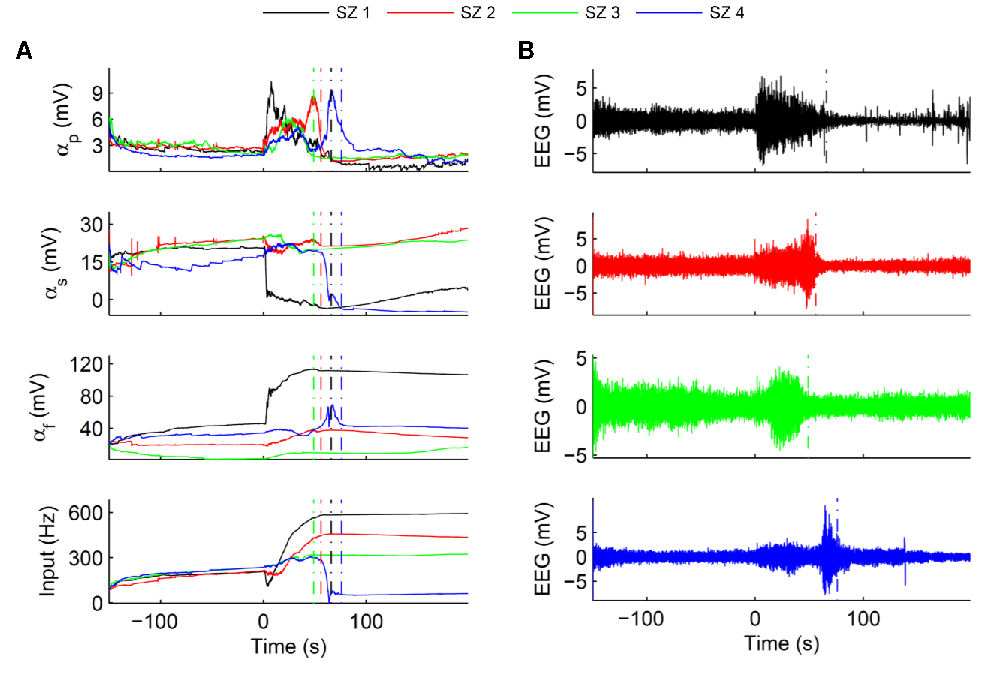
\includegraphics{fig/AnimalComp.pdf}
 	\caption{Estimation Results for Multiple Animals and Simulated EEG. (\textbf{A}) The results from seizures for four different animals. The estimated physiological parameters from each animal (An.) is specified by a different color line. All seizures initiate at time 0s and end at the dotted line that is the same color as the estimation results for the animal. (\textbf{B}) Artificial EEG generated using the neural mass model of the hippocampus. The artificial EEG is generated using the parameters from \textbf{A} with the same color as the traces in \textbf{B}.}
 	\label{fig: SZComp}
 \end{figure}

%That being said, we have tested the algorithm on noisy simulated data, generated from the model, and have shown that it converges to the true parameter values.

\subsection{Estimation Validation}

To validate the estimation results above, we consider the first estimated seizure from each animal. We perform a forward simulation using the estimated slow states~(Figure~\ref{fig: SZComp}). The results for seizure one from each animal are shown. It is clear from these figures that the estimation technique is capable of reproducing model parameters that simulate data similar to recorded EEG.  

We then compare the simulated model dynamics to the observed data to confirm that the estimated slow states are describing the observed phenomena. In particular, we focus on the time a two second time period at the transition to seizure~(Figure~\ref{fig: EEGComp}).

\begin{figure}[ht]
 	\centering
 		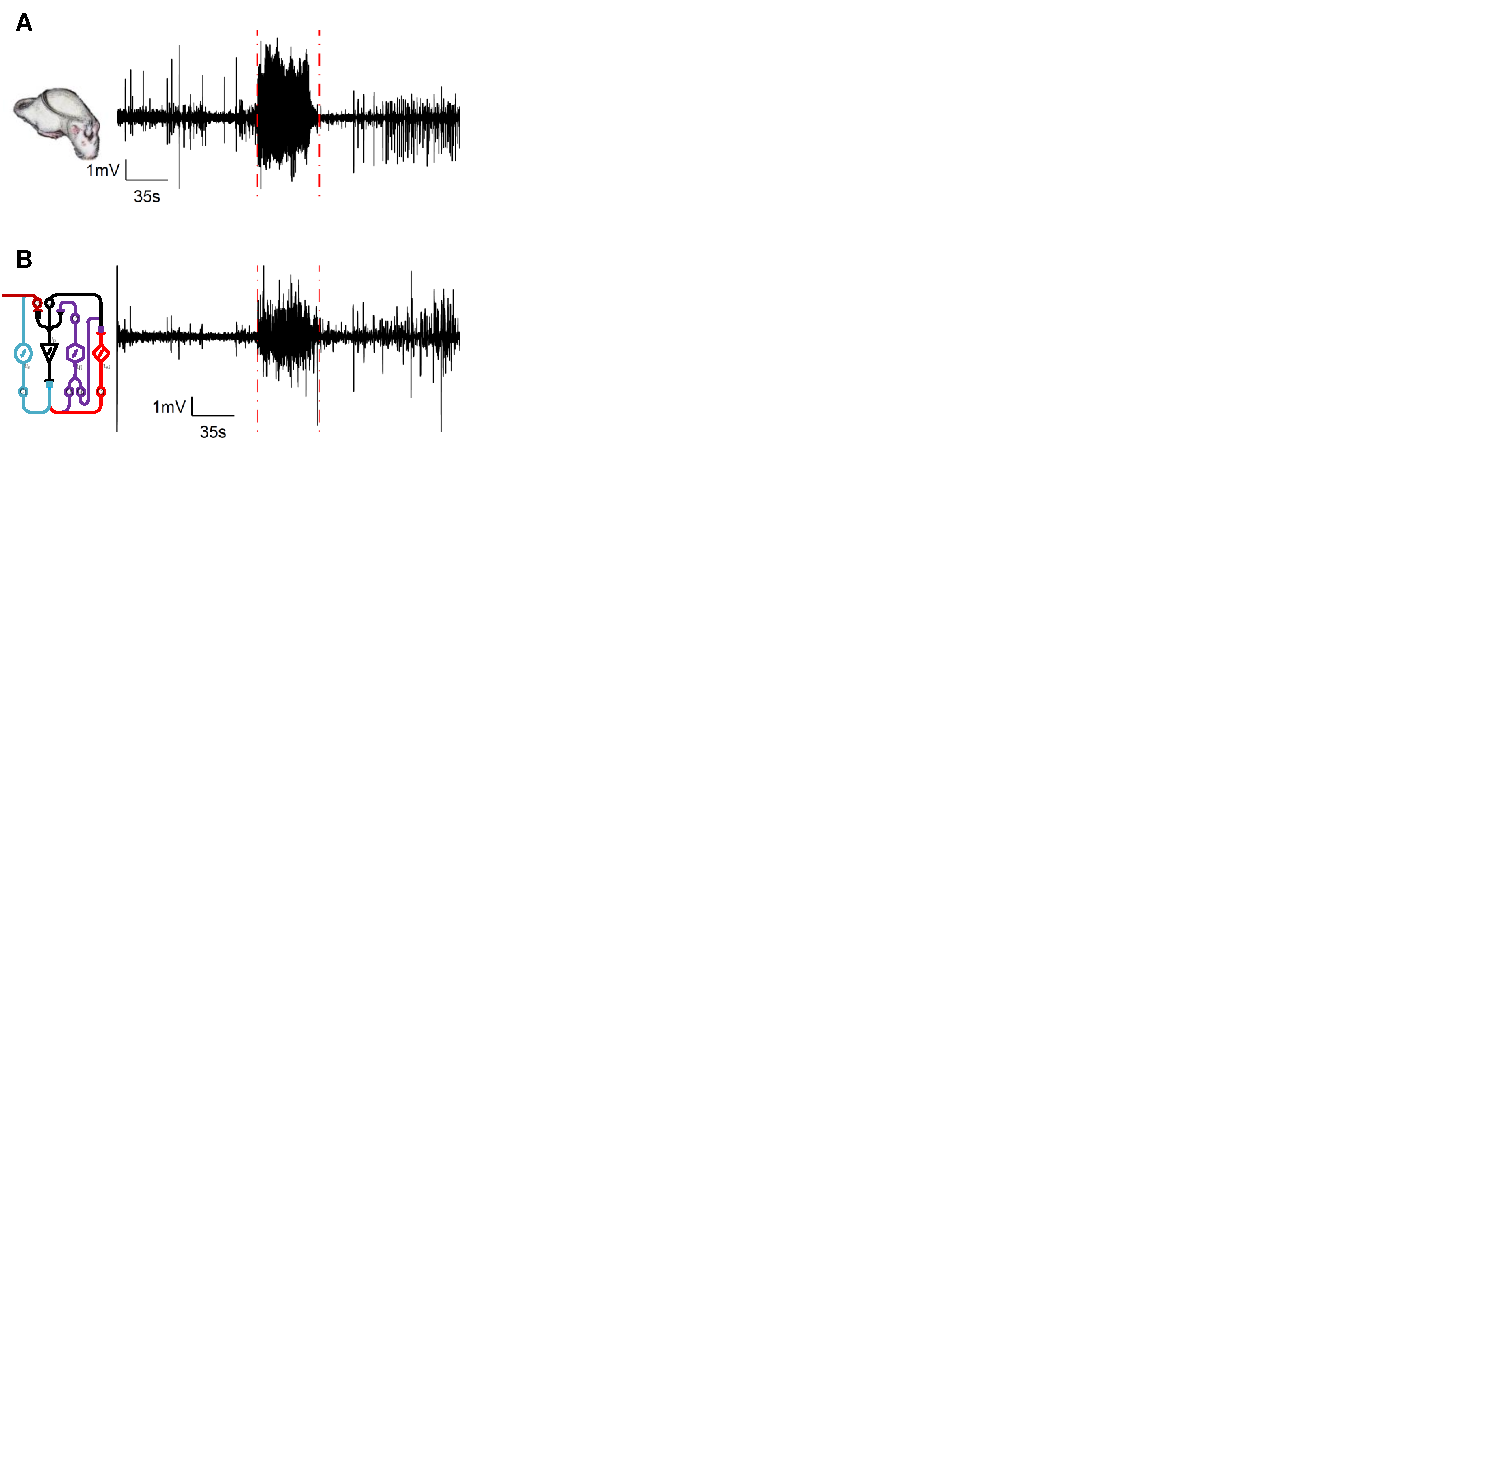
\includegraphics{fig/EEGComparison.pdf}
 	\caption{Recorded and Simulated EEG. (\textbf{A}) Recorded EEG from seizure one of the four different animals (estimation results shown in Figure~\ref{fig: SZComp}). (\textbf{B}) Artificial EEG generated using the neural mass model of the hippocampus. The artificial EEG is generated using the parameters from Figure~\ref{fig: SZComp}.\textbf{A} with the same color as the traces in \textbf{B}. The purple dashed lines indicate the two second time period that has been zoomed into to generate the subfigures in the top right pane. These periods are chosen based on the transitions to seizure for the simulated EEG.}
 	\label{fig: EEGComp}
 \end{figure}

Figure~\ref{fig: EEGComp} demonstrates that the the simulated EEG using the estimated model parameters can replicate similar dynamics to that observed in the recorded EEG. However, there are clear differences between the recorded and simulated EEG. This is clear from considering the zoomed in two second time period. There are clear similarities between the two results as well, and the fact that the simulated EEG transitions to seizure in a similar time frame to the recorded EEG demonstrates the ability of the algorithm to track quickly changing dynamics. Another point of interest is the bifurcations that occur in the simulated EEG. To demonstrate these bifurcations the model is simulated again, but in this case the variance of the stochastic input is drastically reduced.

 \begin{figure}[ht]
 	\centering
 		\includegraphics{fig/Bifurcation.pdf}
 	\caption{Simulated EEG with a stochastic input with low variance using the neural mass model of the hippocampus. The artificial EEG is generated using the parameters from Figure~\ref{fig: SZComp}.\textbf{A} with the same color as the traces.}
 	\label{fig: Bifur}
 \end{figure}

The results from the forward model simulation with a stochastic input with low variance demonstrates the bifurcations that occur in the model using the estimated parameters (Figure~\ref{fig: Bifur}). The black and red traces shows clear bifurcations at the transition to and from seizure. The green and blue traces on the other hand have less clear bifurcations at seizure transitions. However, there is a clear change in the dynamics, but the resulting amplitude from the simulation remains low. After a short period from the point at which the seizure initiates there is a more drastic change in the simulated dynamics, showing a much clearer bifurcation in both the green and blue traces.  

The results that have been shown thus far have only considered the estimation of a each recorded seizure, once. It is known that the unscented Kalman filter does not guarantee convergence\red{ref}; therefore, we consider the performance of the algorithm when estimating the same recorded data with different initialised slow states.  

To demonstrate how robust the unscented Kalman filter is to the starting values chosen for the estimation we have performed a Monte-Carlo analysis~(Figure~\ref{fig: MonteResults}). In each trace the mean and standard deviation of 100 estimated results using randomly initialised slow states are shown. The results show a higher variance on the fast synaptic inhibition ($\theta_f$) and the mean input firing rate post-seizure. However, the slow inhibitory gain standard deviation is higher pre-seizure. To compare the standard deviation over 100 estimations with the predicted error from the unscented Kalman filter we have plotted both results (Figure~\ref{fig: MonteResults}). The results show that there are similarities between the estimated error, and the error over multiple different initialised parameters. In particular, the estimation results pre-seizure for slow inhibition show a high standard deviation for both the single and Monte-Carlo estimation procedure.

\begin{figure}[ht]
	\centering
		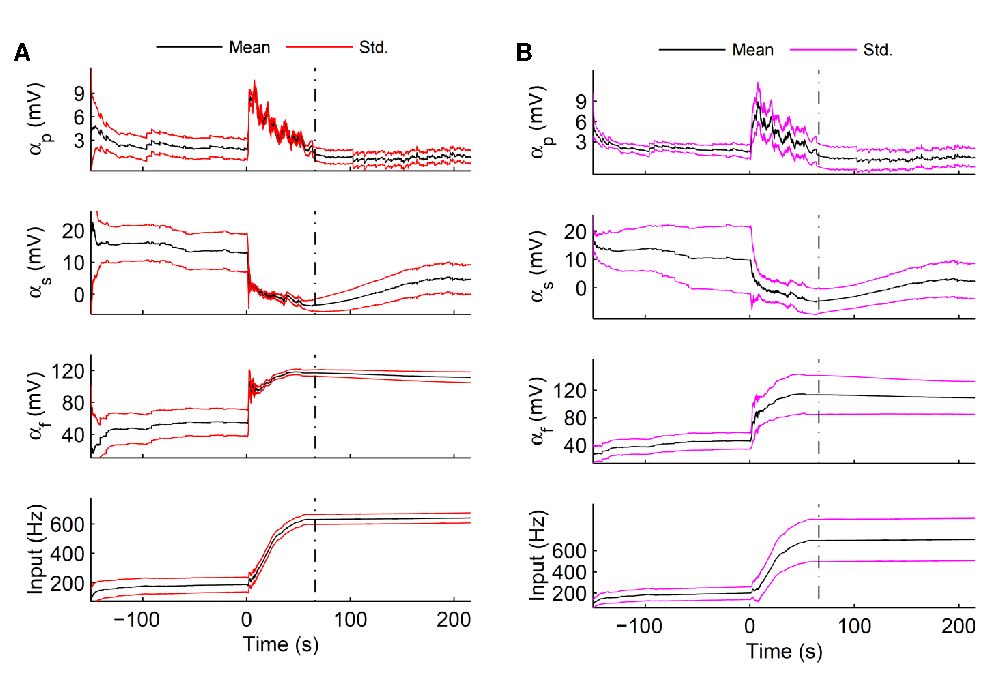
\includegraphics{fig/MonteResults.pdf}
	\caption{Comparison of the mean and standard deviation of a single and monte carlo analysis of the estimation technique. (\textbf{A}) Results from a single estimation are shown, where the standard deviation of each estimate made by the unscented Kalman filter is also shown in red. (\textbf{B}) The mean and standard deviation of 100 estimations using the same data set with different slow states initialised randomly.}
	\label{fig: MonteResults}
\end{figure}

The results from Figure~\ref{fig: MonteResults} also demonstrate the robustness of the unscented Kalman filter to the initialised parameters. In particular, when considering the mean over the Monte-Carlo simulation and the results from a single estimation, there are clear similarities. The transition to and from seizure for all the model parameters have the same trends, and the standard deviation in both sets of results decreases during seizure periods. The Monte-Carlo estimation also shows that there is a higher standard deviation post seizure compared to pre-seizure.
 